{\small
\section{Vererbung}
    \begin{tabular}{ll}
        $\bullet$ & Vererbung funktioniert in Java ähnlich wie in C++\\
        $\bullet$ & Eine Klasse in Java kann jedoch nur \textbf{eine} Basisklasse haben\\
        $\bullet$ & Abgeleitete Klasse erbt Instanzvariablen und Instanzmethoden\\
                  & der Basisklasse\\
        $\bullet$ & Die oberste Klasse aller Basisklassen ist \verb|Object|\\
        $\bullet$ & Methoden von \verb|Object| sind: \\
                  & $\diamond$ \verb|public String toString()| \\
                  & $\diamond$ \verb|public boolean equals(Object obj)| \\
                  & $\diamond$ \verb|public int hashCode()| \\
                  & $\diamond$ ... \\
    \end{tabular}

\columnbreak

\subsection{Impliziter Code in Vererbung}
    \begin{center}
        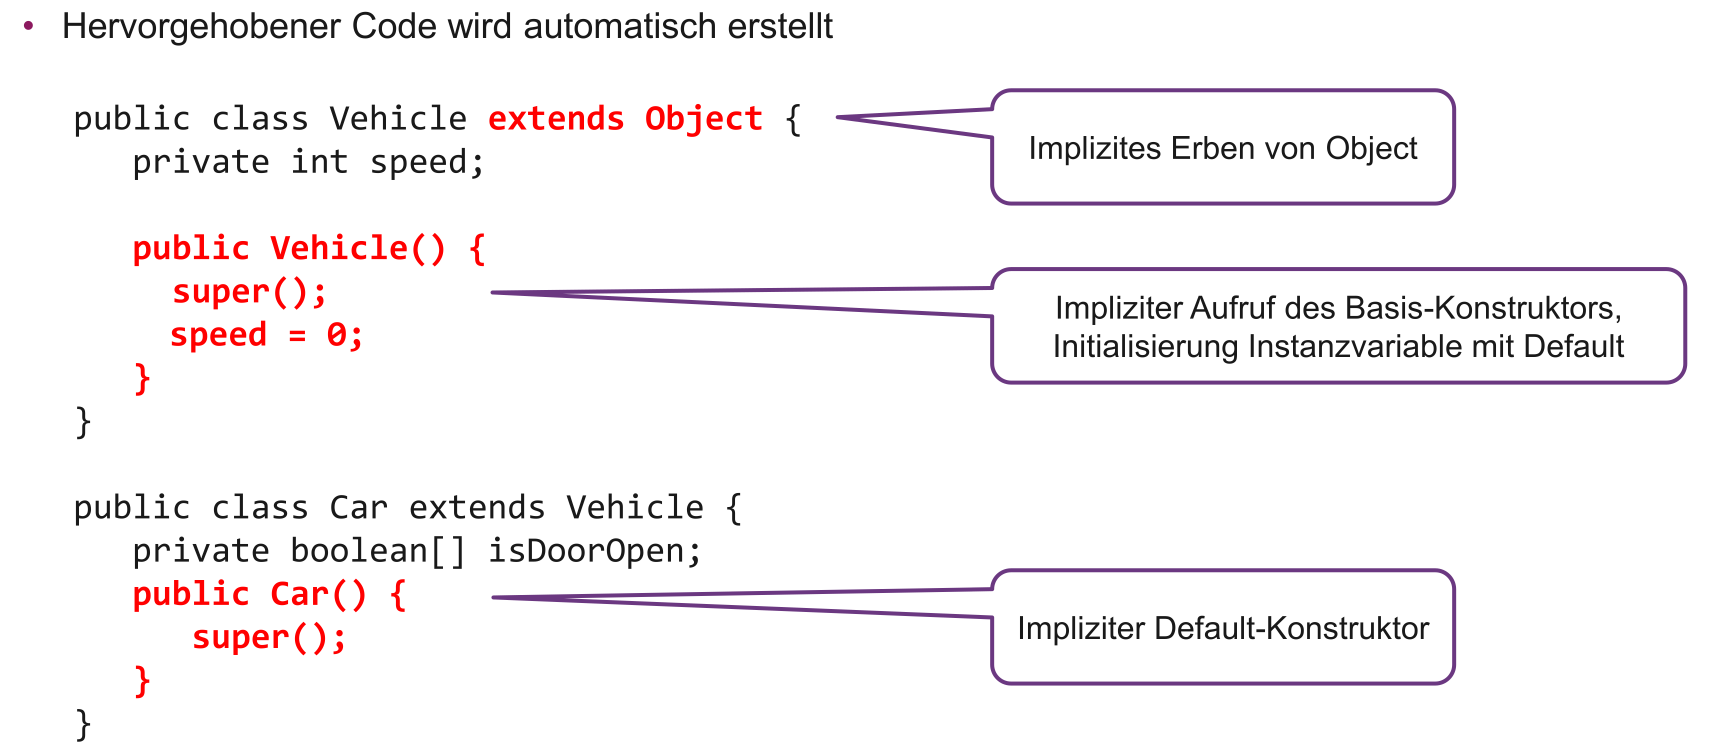
\includegraphics[width=0.9\columnwidth]{pictures/vererbung-implizit.png}
    \end{center}
    \vspace{-0.5cm}

\subsection{Konstruktor bei Vererbung}
    \begin{center}
        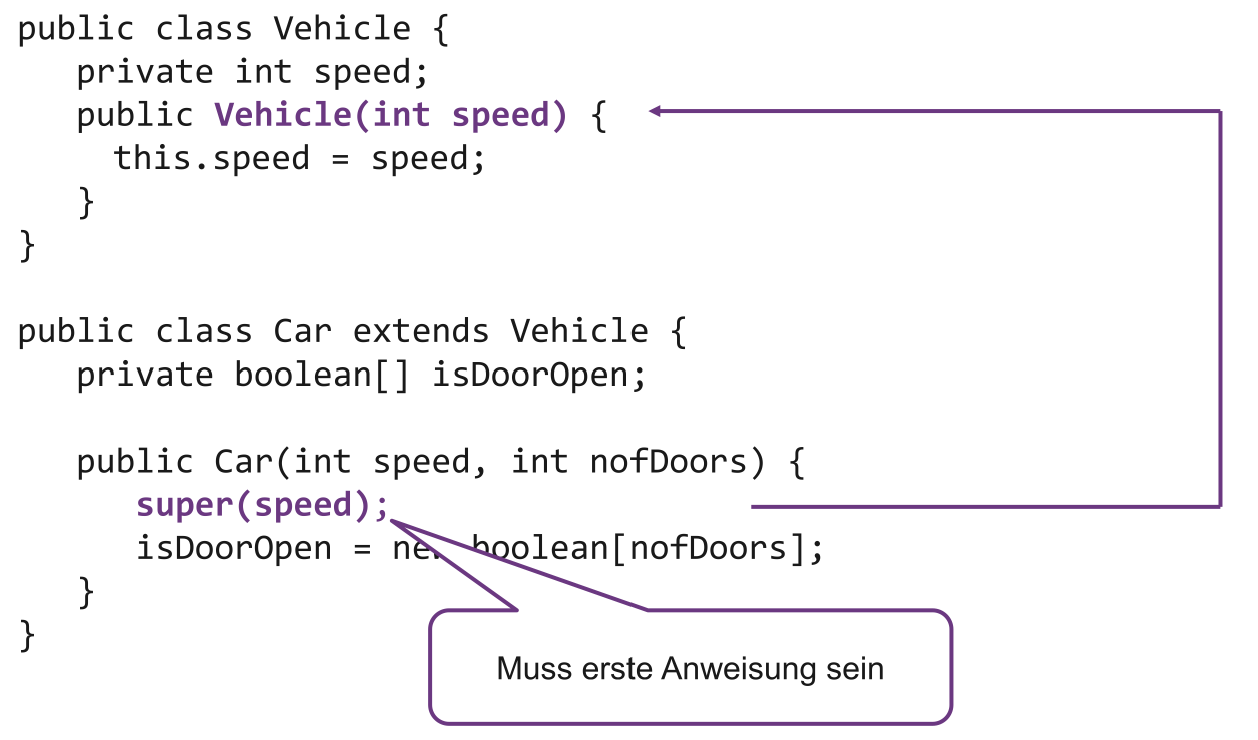
\includegraphics[width=0.7\columnwidth]{pictures/vererbung-konstr.png}
    \end{center}
    \vspace{-0.5cm}

\subsection{Overriden von Methoden}
    Gleiche Funktion wie das Keyword \verb|virtual| in C++, dieses gibt es jedoch nicht in Java. Stattdessen wird
    vor einer neu implementierten Methode einer Subklasse das Schlüsselwort \verb|@Override| gesetzt. Dies ist optional, aber sinnvoll.\\
    \verb|@Override|\\
    \verb|public void print()|\\

    Mit \verb|super| wird eine überschriebene Methode aufgerufen.
    \begin{center}
        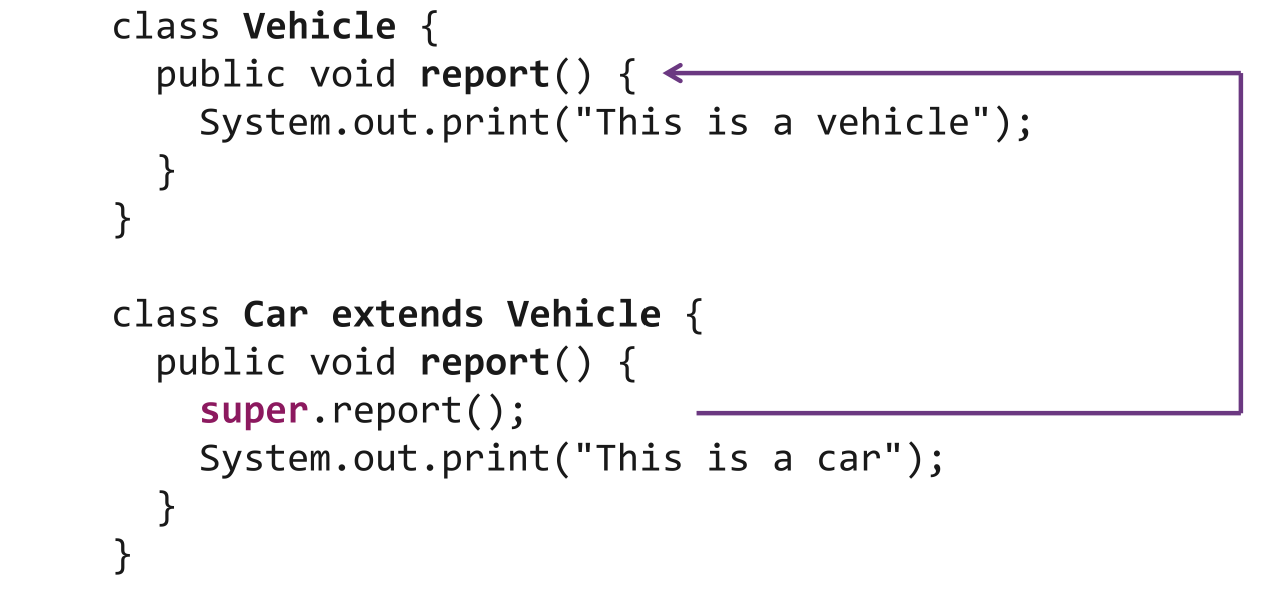
\includegraphics[width=0.7\columnwidth]{pictures/super.png}
    \end{center}
    \vspace{-0.5cm}

\subsection{Abstrakte Klassen $\rightarrow$ abstract}{\label{AbstractClass}}
    \begin{tabular}{l}
        $\bullet$ Eine abstrakte Klasse ist nicht vollständig implementiert,\\
        $\qquad$ sprich einzelne Methoden können nicht implementiert sein\\
        $\bullet$ Die Klasse kann nicht instanziiert werden.\\
        $\bullet$ Dient als Basistyp für Sub-Klassen (statischer Typ)\\
        $\bullet$ Vererbt ihre Grundfunktionalität an Sub-Klassen\\
    \end{tabular}

    \begin{minipage}{0.5\columnwidth}
        \begin{center}
            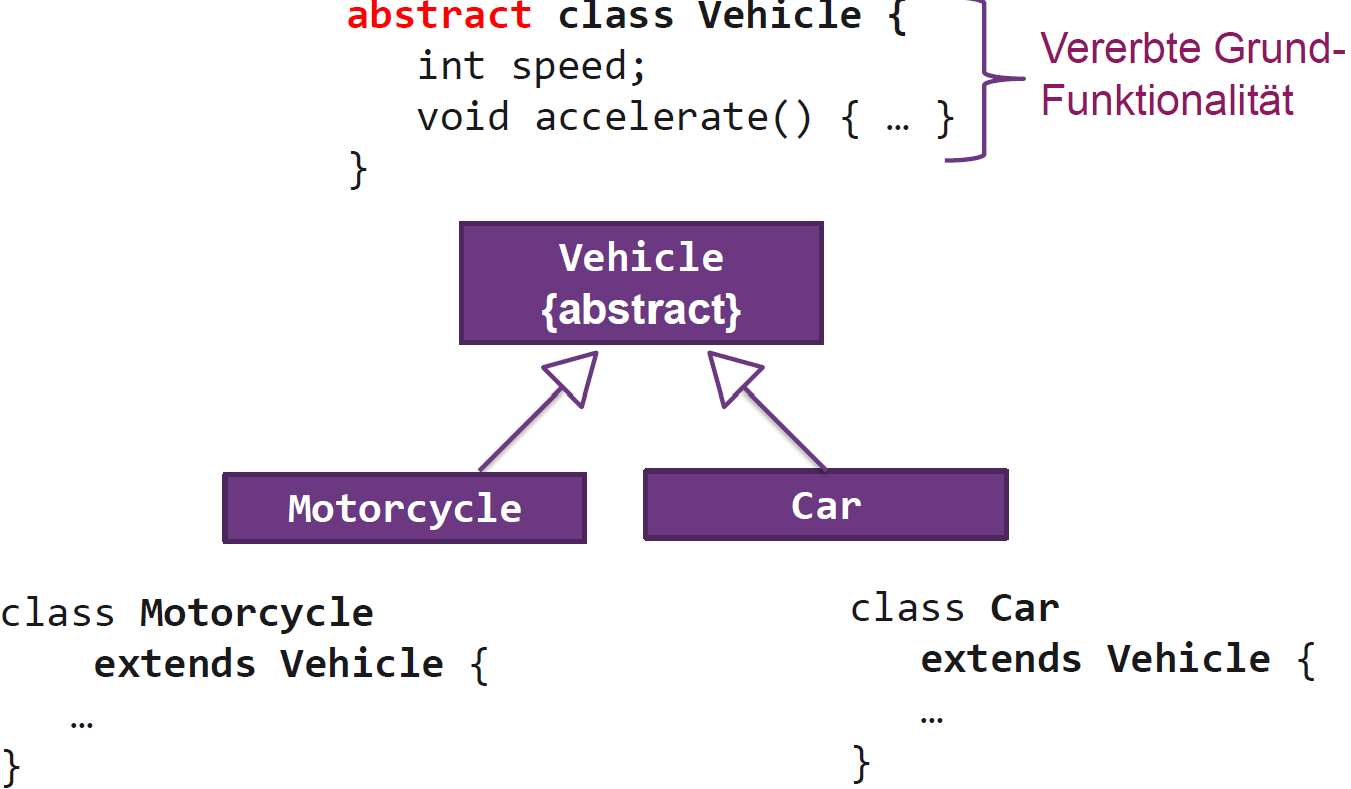
\includegraphics[width=0.9\columnwidth]{pictures/abstrakte-Klasse-Bsp.png}
        \end{center}
    \end{minipage}
    \hfill
    \begin{minipage}{0.5\columnwidth}
        \begin{center}
            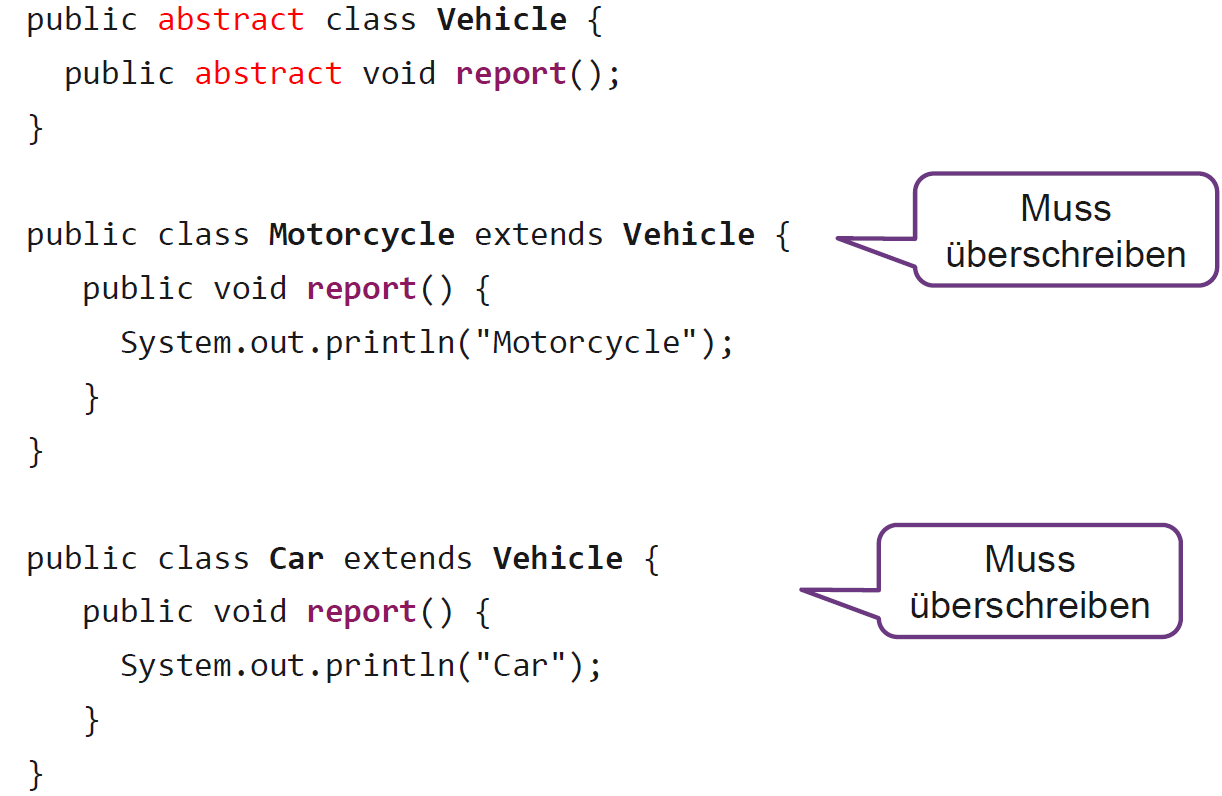
\includegraphics[width=0.9\columnwidth]{pictures/abstrakte-Klasse-Bsp2.png}
        \end{center}
    \end{minipage}
    \vspace{-0.1cm}

\section{Binding}
\subsection{Dynamic Binding}
    Generell bei nicht-privaten Instanzmethoden
    \vspace{-0.1cm}

\subsection{Static Binding}
    Generell bei privaten Instanzmethoden (In Subklasse nicht mehr sichtbar $\rightarrow$ Neudef. der Methode) und statischen Methoden
    \vspace{-0.1cm}
}

